% first presentation about cmtp
\pdfminorversion=4
%\documentclass[ucs]{beamer}
\documentclass{beamer}
%\documentclass[utf8]{beamer}
\usepackage[utf8]{inputenc}
\usepackage{german}
\usepackage{graphicx}
\usepackage{color}
\usepackage{beamerthemesplit}
\usepackage[normalem]{ulem}
%\usepackage{pgf,pgfarrows,pgfnodes,pgfautomata,pgfheaps,pgfshade} 

\setbeamercovered{dynamic}
\usetheme{Malmoe}
\usecolortheme{crane}
\setbeamertemplate{footline}[page number]


\title{Development of a secure, decentralised anonymous chat system}
\subtitle{Bachelor Thesis Presentation}

\author{Nico -telmich- Schottelius}

\date{2012-07-04}

%\pgfdeclareimage[height=0.5cm]{myalias}{pselogo} %declare logo image with an alias here
%\pgfuseimage{myalias}} %use the image right after
\titlegraphic{\includegraphics[width=2cm,height=2cm]{zhaw_logo_de}}


\begin{document}
\frame{\titlepage}

%\section[Outline]{}
\frame{\tableofcontents}

\section{Introduction}
\frame
{
  \frametitle{Who am I?}
  \begin{itemize}
  \item Ex-ETH Sysadministrator, currently Devops-Engineer at local.ch
  \item Long time FOSS developer 
  \item Interested in privacy and anonymity
  \item Last semester student at ZHAW/HSZ-T
  \begin{enumerate}
      \item  Information Security and Cryptography (Informationssicherheit und Kryptografie)
      \item  Networks and Internet Communications (Netzwerke und Internet-Kommunikation)
      \item  Operating Systems (Betriebssysteme)
      \item  Theoretical Computer Science and Automata Theory (Theoretische Informatik und Automatentheorie)
      \item  Scientific Computing (Wissenschaftliches Rechnen)
  \end{enumerate}
  \end{itemize}
}

\frame
{
  \frametitle{Project description}
  \begin{itemize}
  \item Development of a
  \begin{enumerate}
      \item  secure
          \begin{itemize}
          \item Hide message content
          \item Ensure message and sender authenticity
          \end{itemize}
      \item  decentralised
          \begin{itemize}
          \item Flow via different channels
          \item Continue communications even under attack from an enemy
          \end{itemize}
      \item  anonymous
          \begin{itemize}
          \item Hide to whom they are talking to
          \end{itemize}
  \end{enumerate}
  \item chat system
  \end{itemize}
}

\frame
{
  \frametitle{Motivation}
  \begin{itemize}
     \item Client (local.ch, Thomas Gresch)
     \begin{itemize}
        \item Using Skype that, due to its nature, is untrustworthy, but usable
        \item Client seeks for long term replacement 
        \item Sponsors research
    \end{itemize}
     \item Personal
     \begin{itemize}
        \item Support Freedom of Speech
        \item Close the gap between chat systems and anonymity systems (like TOR)
    \end{itemize}
  \end{itemize}
}

\section{Project Planning}
\frame
{
    \frametitle{Status Design Review}
    \begin{center}
    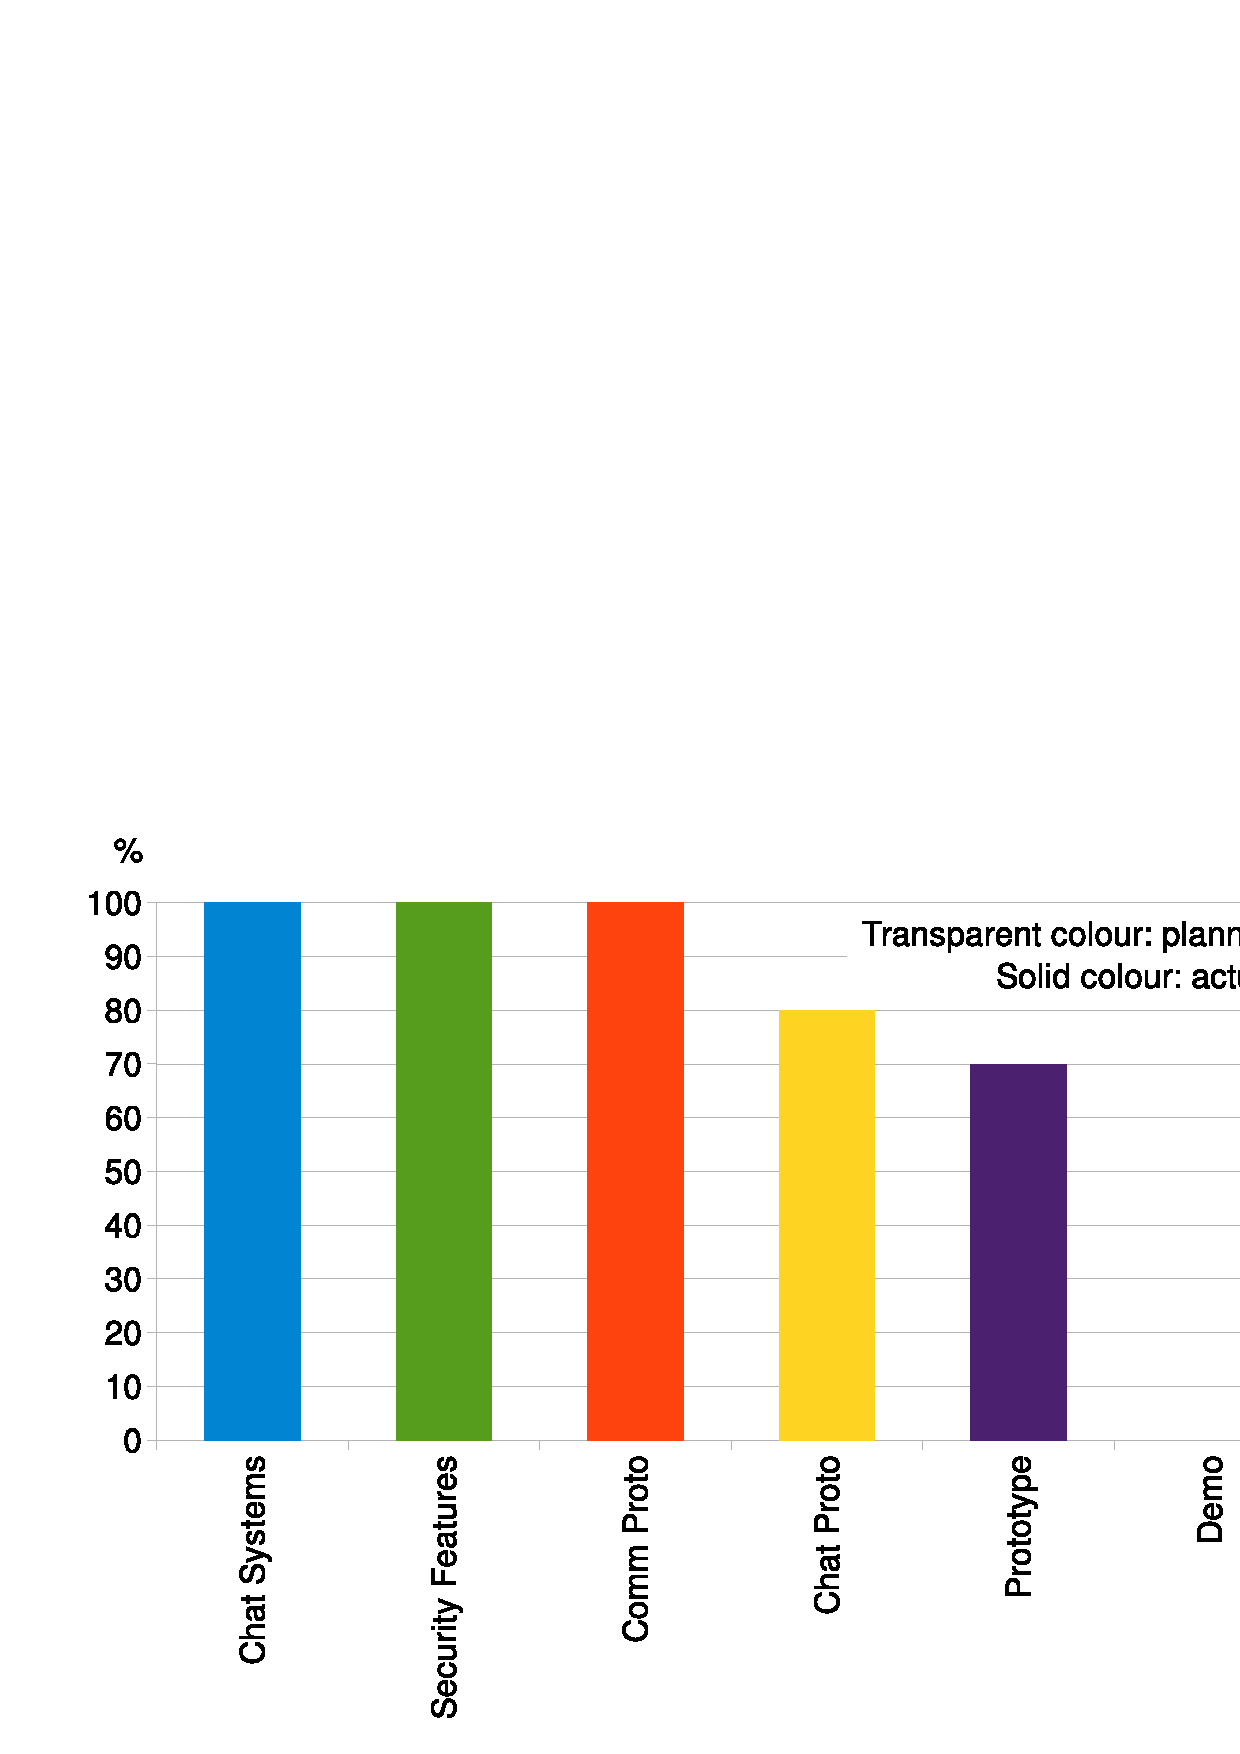
\includegraphics[width=10cm]{status-design-review-percent2.pdf}
    \end{center}
}

\frame
{
    \frametitle{Work after the Design Review}
    \begin{itemize}
    \item Chat Systems: Phrasing cleaned up
    \item Communication Protocols: Added more systems and cleaned up
    \item Security Features: Clarified security related terms
    \item Chat Protocol Definition: Revised many parts, detailed descriptions added
    \item Prototype: Minor enhancements, mostly for tests
    \item Demo: Prepared special scenario and tested
    \end{itemize}
}

\frame
{
    \frametitle{Review Project Planning}
    \begin{itemize}
    \item Started Bachelor Thesis on 2012-03-14 (idea: 2007)
    \item Design Review: 2012-05-19 (\textasciitilde{}70\% finished)
    \item Finished: 2012-06-20 (Presentation: 2012-07-04)
    \item Changed from Chaos to Spiral Model
    \end{itemize}
}

\section{Development Review}
\frame
{
    \frametitle{Skype - Deobfuscated Source Code Website}

    \begin{center}
        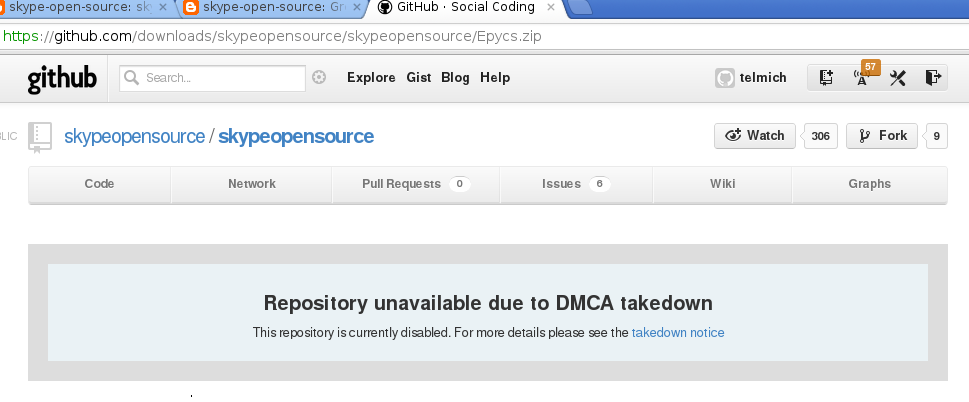
\includegraphics[width=10cm]{dmca-skype.png}
    \end{center}
}

\frame
{
  \frametitle{Security Features}
  \begin{itemize}
          \item Anonymity: Sender-Receiver Anonymity
          \item Confidentiality: Hide message content
          \item Authenticity: Ensure unchanged data and allow sender verification
          \item Availability: Prevent one attacker from shutting down the network
   \end{itemize}
}

\frame
{
  \frametitle{Transport Protocols}
  \begin{itemize}
      \item Multiplexing
      \item Tunneling
      \item Indirect and direct access
  \end{itemize}
  \begin{center}
   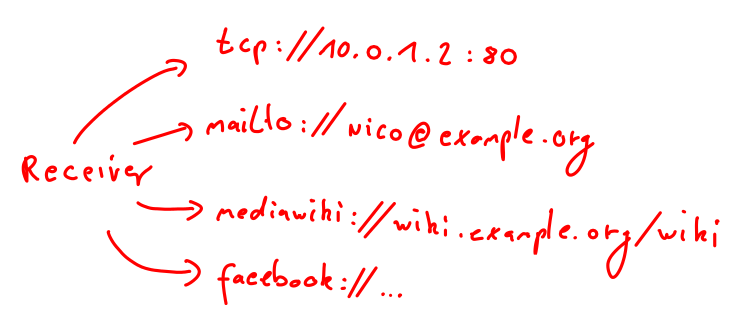
\includegraphics[width=9cm]{../addressmultiplexing.png}
  \end{center}
}

\frame
{
  \frametitle{Onion Routing}
  \begin{itemize}
      \item (Re-)Encrypted for every peer
   \end{itemize}
  \begin{center}
   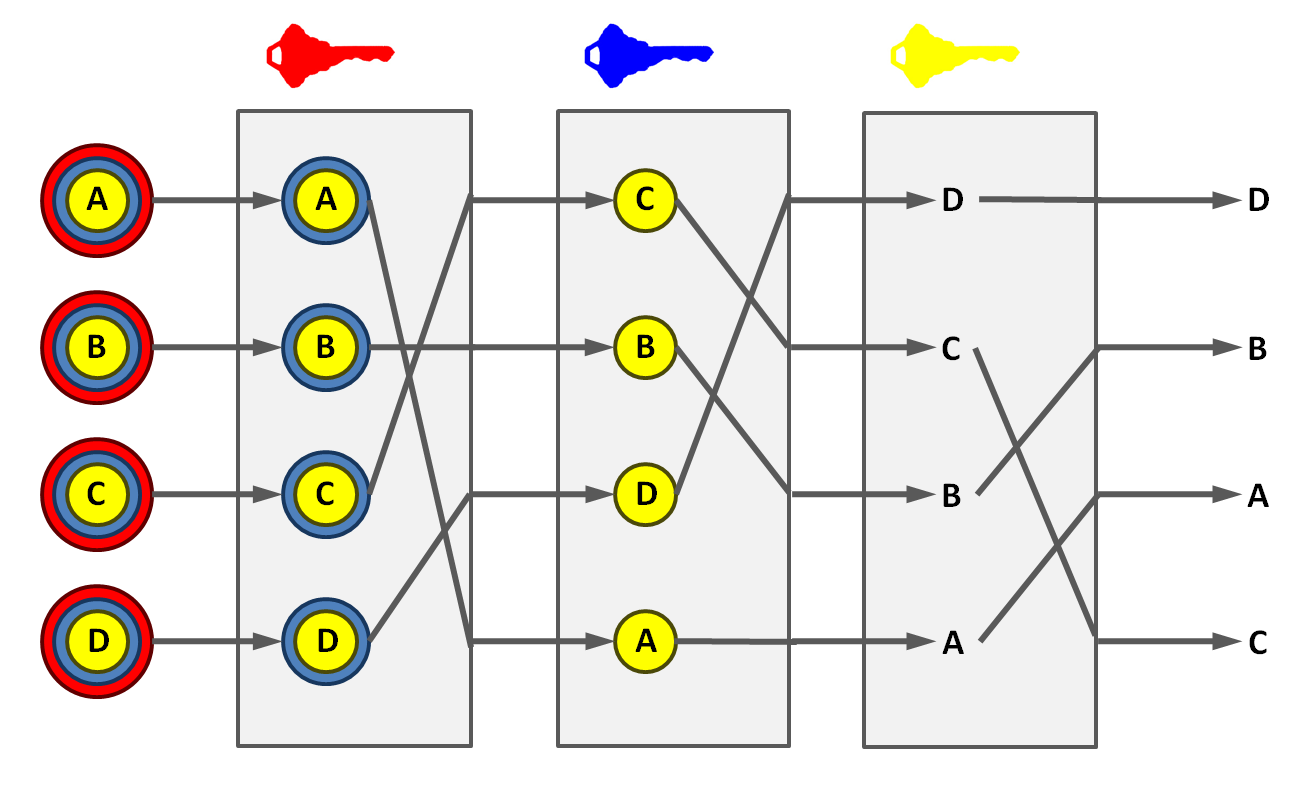
\includegraphics[width=8cm]{../Decryption_mix_net.png}
  \end{center}
}

\frame
{
  \frametitle{Onion Routing (2)}
  \begin{itemize}
      \item Construction of an onion
   \end{itemize}
  \begin{center}
   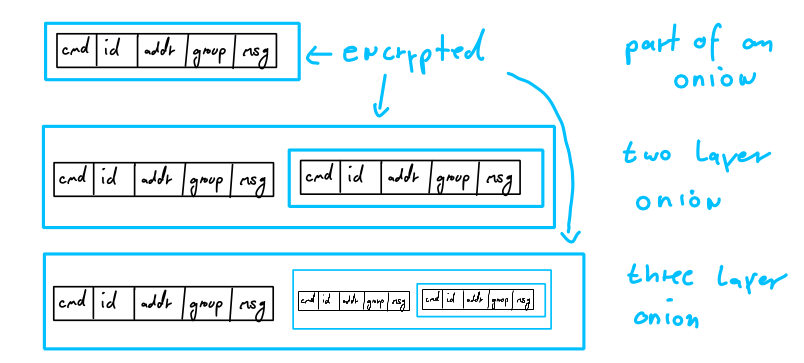
\includegraphics[width=8cm]{../onion.png}
  \end{center}
}

\frame
{
  \frametitle{Onion Routing (3)}
  \begin{itemize}
      \item Receiver is somewhere in the chain
   \end{itemize}
  \begin{center}
   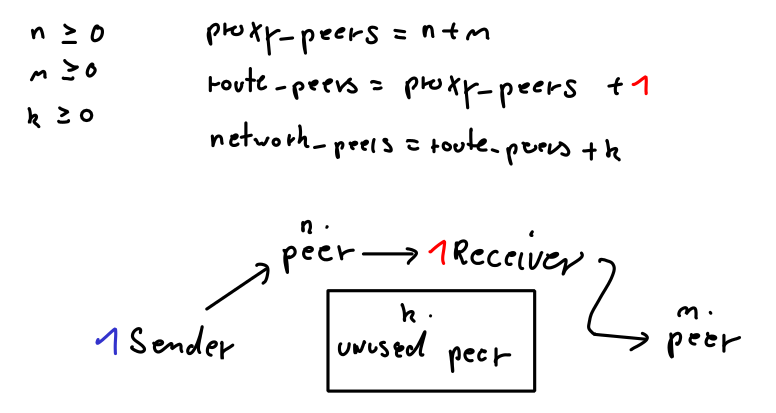
\includegraphics[width=8cm]{../onionrouting.png}
  \end{center}
}

\frame
{
  \frametitle{Noise}
  \begin{itemize}
      \item Prevent statistical analysis
   \end{itemize}
  \begin{center}
   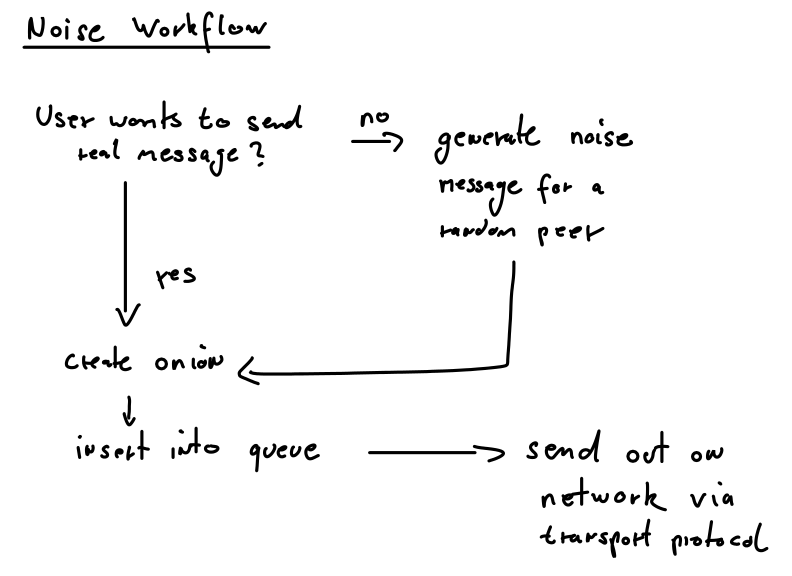
\includegraphics[width=8cm]{../noiseworkflow.png}
  \end{center}
}

%%\frame
%%{
%%  \frametitle{Skype - Deobfuscated Source Code Website}
%%  
%%}

\section{Implementation}
\frame
{
  \frametitle{Prototype}
  \begin{itemize}
     \item Overview
      \begin{itemize}
          \item Python Implementation
          \item Tested with 10 Peers
      \end{itemize}
      \item Components
      \begin{itemize}
          \item Configuration (peer)
          \item Crypto Engine (python-gnupg)
          \item EofID (Base 64 ID String)
          \item EOFMsg (Messages, from protocol)
          \item Noise (Hiding)
          \item Onion (Encapsulation)
          \item Server (Listener, Sender)
          \item Transport Protocol (tcp)
          \item \textit{UI} (Additional code from other project)
      \end{itemize}
   \end{itemize}
}
\frame
{
  \frametitle{Big Picture}
  \begin{center}
   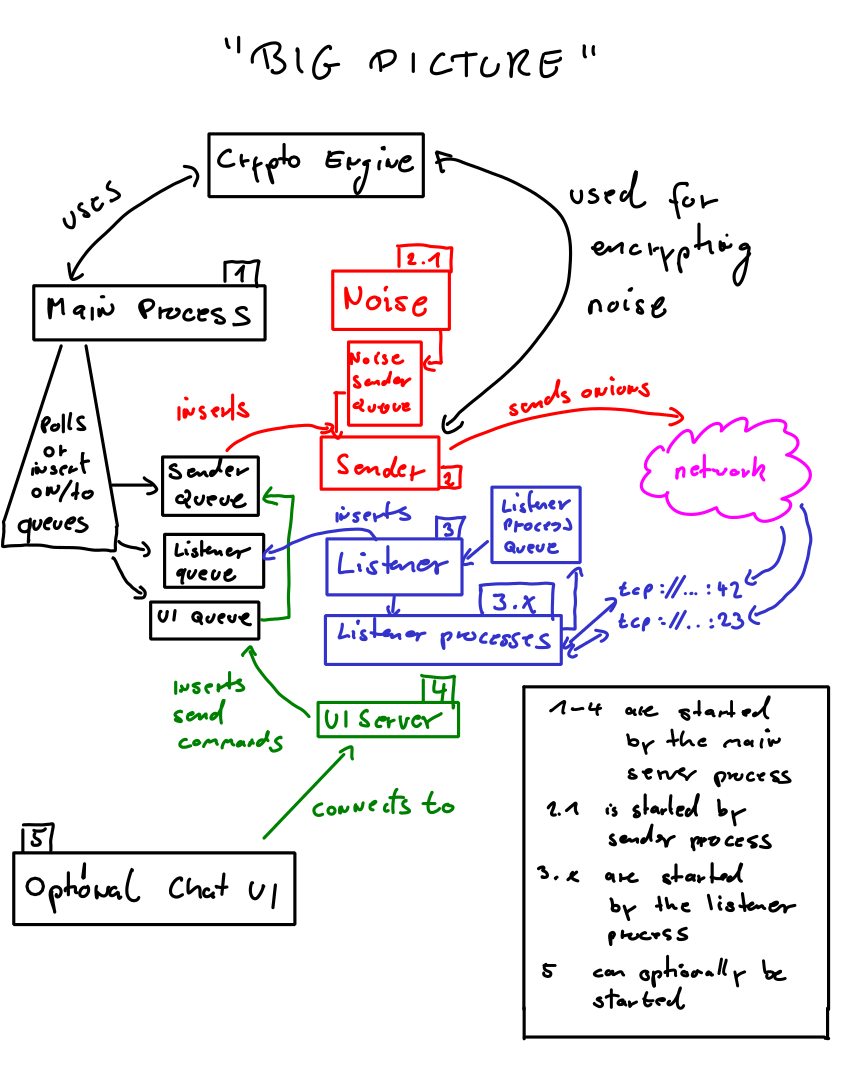
\includegraphics[width=5cm]{../bigpicture.png}
  \end{center}
}

\frame
{
  \frametitle{Test: Bandwidth usage}
  \begin{itemize}
          \item 125ms
          \item 250ms
   \end{itemize}
  \begin{center}
   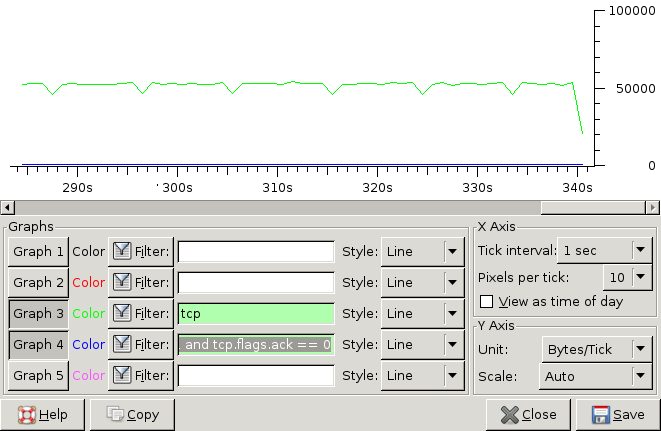
\includegraphics[width=4cm]{../bandwidth-0125.png}
   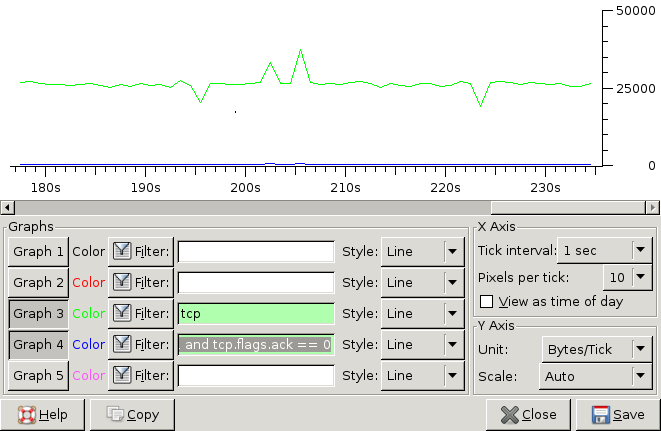
\includegraphics[width=4cm]{../bandwidth-0250.png}
   $$24 KiB/s$$
  \end{center}
}

\frame
{
  \frametitle{Bandwidth usage (network)}
  \begin{center}
   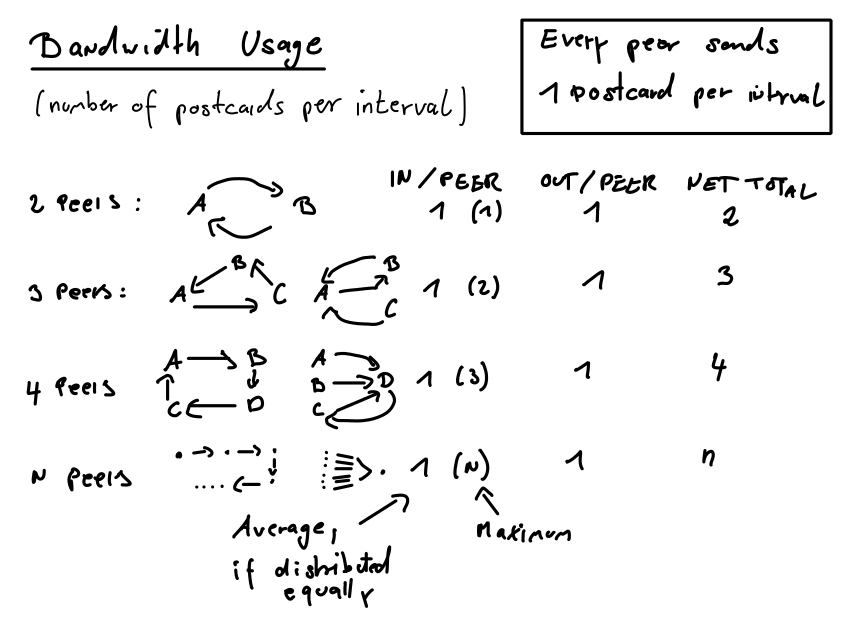
\includegraphics[width=8cm]{../bandwidth.png}
  \end{center}
}

\frame
{
  \frametitle{Test: Performance}
  \begin{itemize}
          \item plain
          \item encrypted
   \end{itemize}
  \begin{center}
   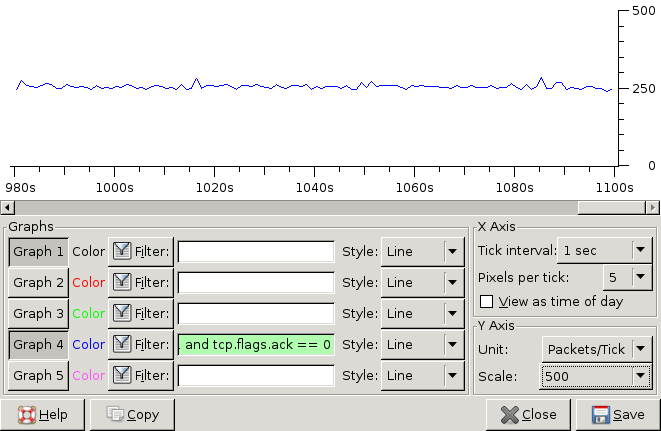
\includegraphics[width=4cm]{../noise-plain-no-limit.png}
   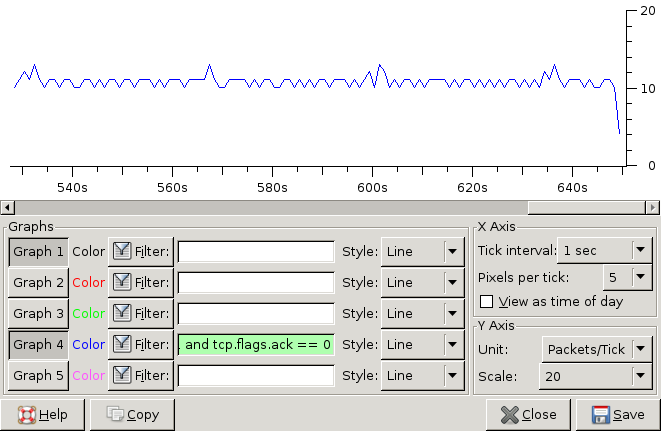
\includegraphics[width=4cm]{../noise-no-limit.png}
   $$10 > 4!$$
  \end{center}
}

\section{Demo}
\frame
{
  \frametitle{Live Demo}
  \begin{itemize}
    \item Send a message
    \item Effect of Noise
  \end{itemize}
}


\section{Conclusions}
\frame
{
  \frametitle{Review Objectives}
\begin{tiny}
\begin{enumerate}
\item Report and comparison of current chat systems including strengths and weaknesses (\alert{done})
\item Report of related communication protocols including strengths and weaknesses (\alert{no strength and weaknesses})
\item Requirement analysis (\alert{focussed on security})
\item Protocol definition paper (containing chat features, data types, transport methods, security measures) (\alert{done})
\item Technical documentation and prototype for the new chat system (\alert{done})
\item Description of test results (\alert{done})
\item Presentation of a successful anonymous, decentralised chat session, which includes proof of the required security by using example attacks (\alert{done})
\end{enumerate}
\end{tiny}

}

\frame
{
  \frametitle{Future Work}
  \begin{itemize}
    \item Authenticity Checks
    \item Key Exchange
    \item Spread Usage
  \end{itemize}
}

\frame
{
  \frametitle{Conclusions}
  \begin{itemize}
    \item Long time research on anonymous system available
    \item Working Prototype created
    \item Chat Protocol defined
    \item A lot of potential to move forward ...
  \end{itemize}
}

\frame
{
  \frametitle{Questions?}
  \begin{center}
  ?
  \end{center}
}

\frame
{
  \frametitle{Backup Slides}
  \begin{center}
  In depth information
  \end{center}
}

\frame
{
  \frametitle{Chat Systems Analysis}
  \begin{itemize}
          \item IRC (Internet Relay Chat): Centralised
          \item SILC (Secure Internet Live Chat): Centralised
          \item XMPP (also know as Jabber): No anonymity
          \item Skype: Untrustworthy, information being censored (DMCA)
   \end{itemize}
}

\frame
{
  \frametitle{Communication Protocols}
    \begin{itemize}
        \item Mix Networks: Original ideas - Used for E-Mail
        \item Tor: No end-to-end anonymity designed
        \item OTR: Short term keys
        \item Freenet: Anonymous file storage
        \item I2P: Non-academic, but interesting anonymous network approach
        \item RUDP: Reliable communication with connection orientation
    \end{itemize}
}

\frame
{
    \frametitle{Status Design Review (Table)}
    \begin{center}
    \begin{tabular}{|c|c|c|c|}
    \hline
    Topic & Planned & Actual & Left\\
    \hline
    Chat Systems & 80\% & 100\% & 20\%\\
    \hline
    Security Features & 80\% & 100\% & 20\%\\
    \hline
    Communication Protocols & 80\% & 100\% & 20\%\\
    \hline
    Chat Protocol Definition & 80\% & 50\% & 20\%\\
    \hline
    Prototype & 0\% & 70\% & 30\%\\
    \hline
    Demo & 0\% & 0\% & 100\%\\
    \hline
    \end{tabular}
    \end{center}
}

\frame
{
  \frametitle{Chat Protocol Definition}
  \begin{itemize}
      \item Details: Data Types 
      \begin{itemize}
          \item Basic: Strings, Encoding
          \item Simple: Commands, Messages, IDs \pause (Demo: base 64 encoding)
          \pause \item Messages
      \end{itemize}
   \end{itemize}
}

\frame
{
  \frametitle{Chat Protocol Definition (2)}
  \begin{itemize}
      \item OpenPGP
      \item Transport Protocols
      \begin{itemize}
          \item Multiplexing
          \item Tunneling
          \item Indirect and direct access
       \end{itemize}
   \end{itemize}
  \begin{center}
   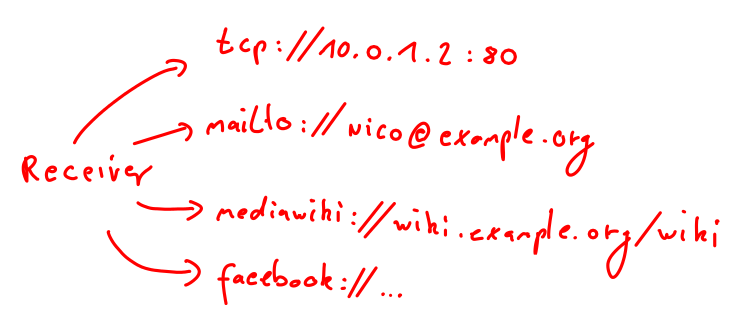
\includegraphics[width=9cm]{../addressmultiplexing.png}
  \end{center}
}

\frame
{
  \frametitle{Chat Protocol Definition}
  \begin{itemize}
    \item Own Base64 transformation (ID)
   \end{itemize}
}

\frame
{
  \frametitle{Tests (Overview)}
  \begin{itemize}
          \item Onion Structure (right order, fields)
          \item Noise Sending (regulary, different peers, different addresses)
          \item Encryption (no plain packets on the wire)
          \item Decryption (all peers can read their message)
          \item Authenticity Verification (\alert{not implemented})
   \end{itemize}
}

\frame
{
  \frametitle{Future Work}
  \begin{itemize}
    \item Authenticity Checks
    \item Verify Cross OS Support
    \item Transport Protocol Support
    \item Impact of decreasing packet size
  \end{itemize}
}


\frame
{
  \frametitle{Future Work (2)}
  \begin{itemize}
    \item Key Exchange
    \item Trust Levels
    \item Multi User Chat
    \item Spread Usage
  \end{itemize}
}

\frame
{
  \frametitle{Time Spent (estimated)}
    $$(8+6) = 14$$
    $$(0+5+5+0+0+7+7)*14 = 336$$
}



% -----------------------------------------------------------------------------
%% \frame
%% {
%%   \frametitle{Agile methods}
%%   \begin{itemize}
%%     \item 
%%       We are uncovering better ways of developing software by doing it and helping others do it. Through this work we have come to value:
%%       Individuals and interactions over processes and tools
%%       \begin{itemize}
%%       \item Working software over comprehensive documentation
%%       \item Customer collaboration over contract negotiation
%%       \item Responding to change over following a plan
%%       \item That is, while there is value in the items on the right, we value the items on the left more.
%%       \end{itemize}
%%     \item Agile Manifesto
%%   \end{itemize}
%% }
%% 
%% 
%% \frame
%% {
%%   \frametitle{Current Situation}
%%   \begin{itemize}
%%       \item Various chat systems available
%%       \begin{itemize}
%%           \item Identifiable who you are talking to (irc, silc, icq, skype?)
%%           \item Centralised (irc, silc, icq, skype partly)
%%           \item Insecure (irc partly, icq)
%%           \item Unknown (skype)
%%       \end{itemize}
%%       \item Client using Skype, closed source, encrypted, proprietary chat system
%%   \end{itemize}
%% }

%\frame
%{
%  \frametitle{Expected Results}
%  \begin{itemize}
%    \item Report and comparison of current chat systems including strength and weaknesses
%    \item Requirement analysis
%    \item Report of related communication protocols including strength and weaknesses
%  \end{itemize}
%}
%\frame
%{
%  \frametitle{Expected Results (2)}
%  \begin{itemize}
%     \item Protocol definition paper (containing chat features,
%        data types, transport methods, security measures)
%    \item Implementation of a prototype for the new chat system
%    \item Presentation of a successful anonymous, decentralised chat session, which
%       includes proof of the required security by using example attacks
%  \end{itemize}
%}

%\section{Objectives}
%\frame
%{
%  \frametitle{Objectives}
%  \begin{itemize}
%    \item Gain deep understanding of routing, anonymity and encryption
%    \item Find out whether targets are realistic
%    \item If so, \pause proof of concept implementation
%  \end{itemize}
%}

%% \frame
%% {
%%   \frametitle{Tor}
%%   \begin{itemize}
%%     \item Anonymous access to resources (web pages)
%%     \item Encrypted transportation, unencrypted after exit node
%%     \item "`It focuses only on protecting the transport of data."' (tor website)
%%     \item Here: Different scenario: closed network, no exit nodes (only chatters)
%%   \end{itemize}
%% }
%% 
%% \frame
%% {
%%   \frametitle{Privacy, Security and Anonymity}
%%     \begin{center}
%%     \includegraphics[scale=0.5]{privacy-security-anon1-300x253.jpg}\footnote{From \url{http://www.concurringopinions.com/archives/2011/01/privacy-vs-security-vs-anonymity.html}}
%%     \end{center}
%% }
%% 
%% \frame
%% {
%%   \frametitle{Project planning: Chaos model}
%%   \begin{enumerate}
%%      \item Resolve the most important issue first\footnote{See \url{http://en.wikipedia.org/wiki/Chaos_model}}
%%      \item An issue is an incomplete programming task.
%%       \begin{enumerate}
%%          \item The most important issue is a combination of big, urgent, and robust.
%%          \item Big issues provide value to users as working functionality.
%%          \item Urgent issues are timely in that they would otherwise hold up other work.
%%          \item Robust issues are trusted and tested. Developers can then safely focus their attention elsewhere.
%%       \end{enumerate}
%%      \item To resolve means to bring it to a point of stability.
%%   \end{enumerate}
%% }
%% 
%% \frame
%% {
%%   \frametitle{Dates}
%%   \begin{itemize}
%%      \item Kick-Off: 2012-03-14
%%      \item Design-Review: End of April
%%      \item Defense: End of June
%%   \end{itemize}
%% }

%% \section{Conclusions}
%% \frame
%% {
%%   \frametitle{Projectphases and Dates}
%%   \begin{itemize}
%%      \item Kick-Off: 2012-03-14
%%       \begin{itemize}
%%          \item Current state analysis
%%          \item Initial protocol design
%%       \end{itemize}
%%      \item Design-Review: \sout{End of April} \alert{2012-05-09}
%%      \begin{itemize}
%%          \item Final protocol design
%%          \item Implementation (including testing) of Prototype
%%      \end{itemize}
%%      \item Final presentation: \sout{End of June} \alert{2012-07-05}
%%   \end{itemize}
%% }


\end{document}
